\documentclass[11pt,a4paper,twoside]{book}
\usepackage{etoolbox}                          % required by \iftoggle
\usepackage[utf8]{inputenc}
% \usepackage{fullpage}                        % Widen page margin
\usepackage{amsmath}
\usepackage{amsfonts}
\usepackage{amssymb}
\usepackage{graphicx}
\usepackage{lmodern}
\usepackage{makecell}
\usepackage{lipsum}
\usepackage{ccicons}

\usepackage[colorlinks,linktoc=all]{hyperref}  % Color links
\usepackage[printonlyused,withpage]{acronym}   % Acronyms
\usepackage[usenames,dvipsnames]{color}        % named colors such as CadetBlue
\usepackage{listings}                          % Code synthax highlighting package
\usepackage{lstlang1}                          % C++ settings
\usepackage{courier}

\usepackage[colorinlistoftodos, textwidth=4cm, shadow]{todonotes} % Todo notes
\usepackage{makeidx}

%%%% Hyper-Links Setup %%%
\hypersetup{
    colorlinks,%
    linkcolor=black,%
    citecolor=Orchid,%
%    filecolor=black,%
    urlcolor=CadetBlue
}
%%%%%%%%%%%%%%%%%%%%%%%%%%

%%% Auto-Indexing for Acronyms %%%
\let\oldac\ac
\renewcommand*{\ac}[1]{\oldac{#1}\index{#1}}
%%%

%%% Code Color Coding %%%
\definecolor{lightgray}{rgb}{0.95,0.95,0.95}

%\lstloadlanguages{[ISO]C++, Java}
% Check Dokumentation for further languages ...
         %[Visual]Basic
         %Pascal
         %C

         %XML
         %HTML
 %        Java
% }
\lstset{
	language=[ISO]C++,
	basicstyle=\footnotesize\ttfamily, 
	extendedchars=true,         
	breaklines=false,            
	keywordstyle=\color{MidnightBlue}\bfseries, 
	commentstyle=\color{LimeGreen},
	stringstyle=\color{Orchid}\ttfamily, 
	morekeywords={boolean, octet, wchar, string, wstring, sequence, fixed,}
}  
	
%%\lstset{
%%		 language=[ISO]C++,
%%         basicstyle=\footnotesize\ttfamily, 
%%%         numbers=left,               
%%         numberstyle=\tiny,          
%%%         stepnumber=2,               
%%%         numbersep=5pt,              
%%         tabsize=2,                  
%%         extendedchars=true,         
%%%         breaklines=false,            
%%         keywordstyle=\color{BrickRed}\bfseries, 
%%         frame=b,         
%% %        keywordstyle=[1]\textbf,    
%% %        keywordstyle=[2]\textbf,    %
%% %        keywordstyle=[3]\textbf,    %
%% %        keywordstyle=[4]\textbf,
%%% 
%%   		 commentstyle=\color{LimeGreen},   
%%%   		 morecomment=[l][\color{Gray}]{//},
%%%   		 morecomment=[s][\color{Gray}]{/*}{*/}, 
%%%   		 morestring=[b][\color{OliveGreen}]{"},
%%%   		 classoffset=0,

%%%   		 morekeywords={int,long, char, float, double},keywordstyle=\color{RubineRed},classoffset=1,
%%%   		 morekeywords={for, if, while, catch, throw, break, switch, new, delete, namespace},keywordstyle=\color{RoyalPurple},
%%%   		 classoffset=0,
%%         stringstyle=\color{Orchid}\ttfamily, 
%%         showspaces=false,           
%%         showtabs=false,             
%%         xleftmargin=17pt,
%%         framexleftmargin=17pt,
%%         framexrightmargin=5pt,
%%         framexbottommargin=4pt,
%%         %backgroundcolor=\color{lightgray},
%%         showstringspaces=false      
% }
 
    %\DeclareCaptionFont{blue}{\color{blue}} 

  %\captionsetup[lstlisting]{singlelinecheck=false, labelfont={blue}, textfont={blue}}
  \usepackage{caption}
\DeclareCaptionFont{white}{\color{white}}
\DeclareCaptionFormat{listing}{\colorbox[cmyk]{0.43, 0.35, 0.35,0.01}{\parbox{\textwidth}{\hspace{15pt}#1#2#3}}}
\captionsetup[lstlisting]{format=listing,labelfont=white,textfont=white, singlelinecheck=false, margin=0pt, font={bf,footnotesize}}

%%%%%%%%%%%%%%%%%%%%%%%%%%%%%%%%%%%%%%%%%%%%%%%%%%%%%%%%%%%%%%%%%%%%%%%%

%%%%%%%%% Programming Language Toggles
\newtoggle{cpp}
\newtoggle{java}
\newtoggle{scala}

%% Define toggle for the programming language
\toggletrue{cpp}
\togglefalse{java}
\togglefalse{scala}


\author{
	Angelo Corsaro\\ 
	Chief Technology Officer\\
	PrismTech\\
	\href{mailto:angelo.corsaro@prismtech.com}{angelo.corsaro@prismtech.com}
}
\title{ \huge The Data Distribution Service Tutorial}
\date{}
\makeindex

\begin{document}
% \listoftodos
\maketitle

\thispagestyle{empty}

%%% Copyright %%%
\pagestyle{empty}
%% copyrightpage
\begingroup
\footnotesize
\parindent 0pt
\parskip \baselineskip
% \cc \ccby \ccnc \ccsa PrismTech, 2014 \\
\ccbysa{}  PrismTech, 2014 \\
\newline
\textcopyright{} 2014 by PrismTech.  This work is made available under a Creative Commons Attribution-Share Alike 4.0 License (international) \\
\href{http://creativecommons.org/licenses/by-sa/4.0}{http://creativecommons.org/licenses/by-sa/4.0}

    The Current Maintainer of this work is \href{mailto:angelo@icorsaro.net}{Angelo Corsaro}

%    \lipsum[1-2]

\begin{center}
\begin{tabular}{ll}
First edition:  & May 2014 \\
\end{tabular}
\end{center}
%
%\vfill
%
%Bobs, Ju.\\
%\hspace*{2em} Me, myself, and I / Jubobs. -- \\
%\hspace*{1em} Toilet-paper Press ed. \\
%\hspace*{2em} p. \hspace*{2em} cm. \\
%\hspace*{2em} Includes illustrations, bibliographical references and index. \\
%\hspace*{2em} ISBN \\
%\hspace*{2em} 1. Book design \hspace*{2em} I. Title
%
%
%\vfill
%
%The Toilet Paper Press, \\
%Portland, OR \\
%\texttt{toiletpaper dot press (at) jubobs dot com}

%%%%{\LARGE\plogo}
\vspace*{2\baselineskip}


\endgroup
\clearpage
%%%

\pagestyle{headings}
\setcounter{page}{1}
\pagenumbering{roman}
\tableofcontents
\setcounter{page}{1}
\pagenumbering{arabic}
\chapter{Foundations}\label{Chapter:Foundations}
\section{The Data Distribution Service}\label{Section:Intro}
Whether you are an experienced programmer or a newbie, it is highly likely 
that you have already experienced some form of \ac{Pub/Sub} -- 
%%
%%\todo[inline, caption={Actualize Intro}]{The description of DDS should be updated 
%% to put more emphasis on data sharing. I addition we should have some quick reference 
%% to MQTT, JMS,~\ldots}
%%
an abstraction for one-to-many communication that provides anonymous, 
decoupled,  and asynchronous communication between the publisher and 
its subscribers. \ac{Pub/Sub} is the abstraction behind many of the technologies 
used today to build and integrate distributed applications, such as, social 
application,  financial trading, etc., while maintaining their 
composing parts loosely coupled and independently evolvable.

Various implementations of the \ac{Pub/Sub} abstraction have emerged through time to 
address the needs of different application domains. \ac{DDS} is an \ac{OMG} 
standard for \ac{Pub/Sub} introduced in 2004 to address the data sharing needs 
of large scale mission- and business-critical applications. Today \ac{DDS} is 
one of the hot technologies at the heart of some of the most interesting \ac{IoT} and 
\ac{I2} applications.
 
At this point, to the question "What is DDS?" I can safely answer that it is 
a \ac{Pub/Sub} technology for ubiquitous, polyglot, efficient and secure data sharing. 
Another way of answering this question is that \ac{DDS} is \ac{Pub/Sub} on \textit{steroids}.


\section {The OMG DDS Standard}
The \ac{DDS} standards family is today composed, as shown in
Figure~\ref{Figure:DDS:Standard}, by the 
\ac{DDS} v1.2 API \cite{OMG:DDS:04} and the \ac{DDSI} (\ac{DDSI} v2.1) \cite{OMG:DDSI:06}. 
% \todo[inline, caption={Standard References}]{Standard References are out of date.}
The \ac{DDS} API standard guarantees source code portability across different vendor 
implementations, while the \ac{DDSI} standard ensures on the wire interoperability 
between DDS implementations from different vendors. The \ac{DDS} API standard defines several  different profiles (see Figure~\ref{Figure:DDS:Standard}) that enhance 
real-time pub/sub with content filtering and queries, temporal decoupling and automatic fail-over. 
%%
\begin{figure}[ht]
	\centering
	\includegraphics[scale=0.4]{figs/dds-standard.eps}
	\caption{The \ac{DDS} Standard.}
	\label{Figure:DDS:Standard}
\end{figure}
%%

The \ac{DDS} standard was formally adopted by the \ac{OMG} in 2004 and today it has 
become the established \ac{Pub/Sub} technology for distributing high volumes of data, 
dependably and with predictable low latency in applications such as, Smart Grids,
Smart Cities, Financial Trading, Air Traffic Control and Management,  High Performance Telemetry and  Large Scale Supervisory Systems. 

Now that I have given you an overall idea of what \ac{DDS} is and where it is being used 
let's try to see how it works.



\section {\ac{DDS} in  a Nutshell}
To explain \ac{DDS} I will take advantage of a running example that is 
simple and generic enough that you should easily relate to it. 
I will describe the example now and then use it to explain 
the various \ac{DDS} features throughout this tutorial. 
The example that I will use is the temperature monitoring and 
control system for a very large building. Each floor of 
the building has several rooms, each of which is equipped with 
a set of temperature and humidity sensors and one or more conditioners. 
The application is supposed to perform both monitoring for all the 
elements in the building as well as temperature and humidity control 
for each room. 

This application is a typical distributed monitoring and control 
application in which you have data telemetry from several sensors 
distributed over some spatial location and you also have the control 
action that has to be applied to the actuators--our conditioners. 

Now that we've created a task for you to solve, let's see what \ac{DDS} 
has to offer.

\subsection{Global Data Space}\index{Global Data Space}
The key abstraction at the foundation of \ac{GDS} is a fully 
distributed {\ac{GDS}. It is important to remark that the \ac{DDS} 
specification requires the implementation of the Global Data Space 
to be fully distributed to avoid point of failures and single point 
of bottleneck. Publishers and Subscribers can join or leave the \ac{GDS} 
at any point in time as they are dynamically discovered. The dynamic 
discovery of Publisher and Subscribers is performed by the \ac{GDS} 
and does not rely on any kind of centralized registry such as those 
found in other pub/sub technologies such as \ac{JMS}. Finally, 
I should mention that the \ac{GDS} also discovers application defined 
data types and propagates them as part of the discovery process.
%%
\begin{figure}[ht]
	\centering
	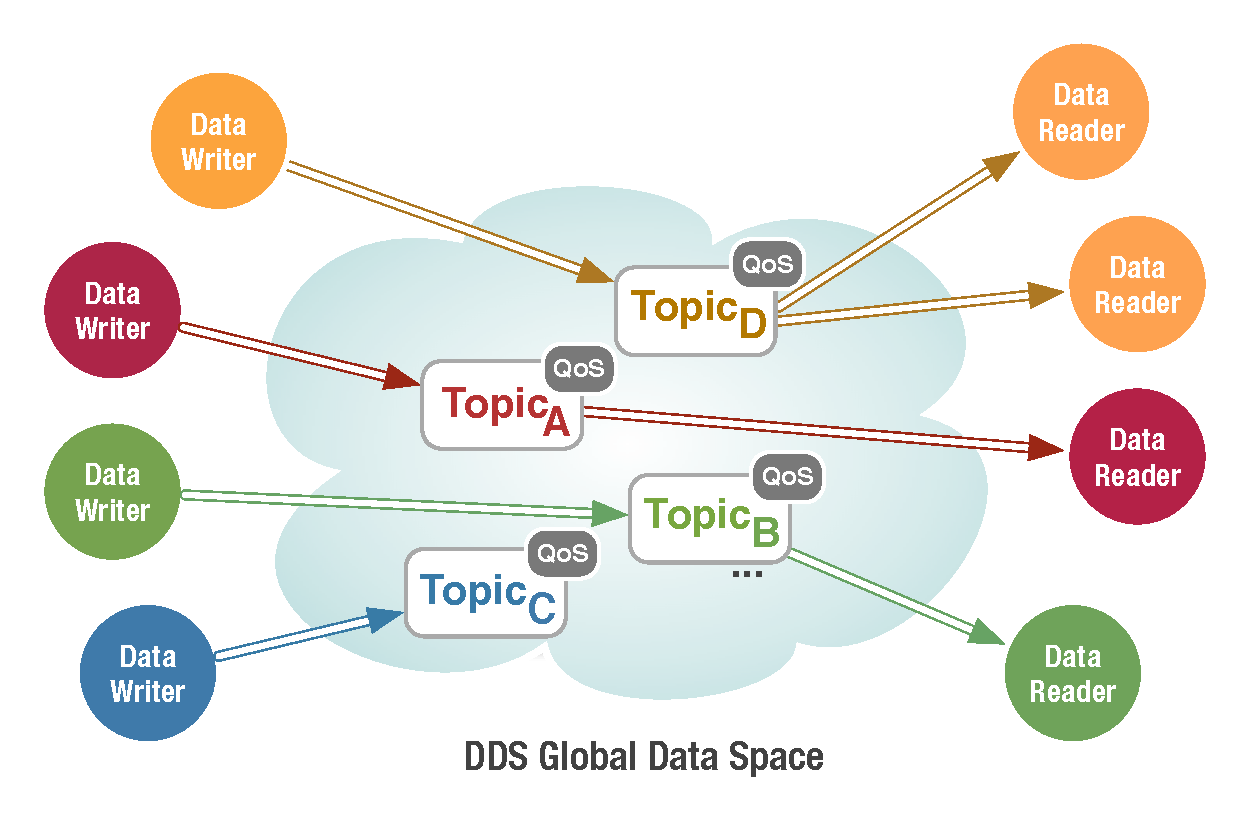
\includegraphics[scale=0.5]{figs/gds.eps}
	\caption{The Global Data Space.}
	\label{Figure:DDS:Standard}
\end{figure}
%%
In essence, the presence of a \ac{GDS} equipped with dynamic discovery 
means that when you deploy a system, you don't have to configure anything. 
Everything will be automatically discovered and data will begin to flow. 
Moreover, since the \ac{GDS} is fully distributed you don't have to fear the 
crash of some server inducing unknown consequences on the system 
availability -- in DDS there is no single point of failure, although 
applications can crash and restart, or connect/disconnect, the system 
as a whole continues to run.

\subsection{Domain Participants}\index{Domain Participant}
To do anything useful a \ac{DDS} application needs to create a \ac{DP}.
The \ac{DP} gives access to the \ac{GDS} -- called domain in \ac{DDS} applications. 
Listing~\ref{Listing:DDS:CreateDP} shows how a \ac{DP} can be created,
notice that domains are identified by integers.

 %%%
\iftoggle{cpp}{
	\lstinputlisting[
		frame=b,
		label={Listing:DDS:CreateDP},
		caption={Topic creation.}]
		{./listing/cxx/create-dp.cpp}
}

%%%
\iftoggle{java}{
	\lstinputlisting[
		frame=b,
		label={Listing:DDS:CreateDP},
		caption={Topic creation.}]
		{./listing/java/create-dp.java}
}
%%%

\iftoggle{scala}{
	\lstinputlisting[
		frame=b,
		label={Listing:DDS:CreateDP},
		caption={Topic creation.}]
		{./listing/scala/create-dp.scala}
}

\subsection{Topics}
I've evoked several times this vision of the data flowing 
from Publishers to Subscribers. In \ac{DDS} this data belongs to a
Topic \index{Topic} and represents the unit of information that can be produced 
or consumed.  A Topic is defined as a triad composed of a type, 
a unique name, and a set of Quality of Service (QoS) policies which, 
as I'll explain in detail later in this tutorial, are used to control 
the non-functional properties associated with the Topic. 
For the time being it is enough to say that if the \ac{QoS}s are not explicitly set, 
then the \ac{DDS} implementation will use some defaults prescribed by the standard.

Topic Types \index{Topic Types} can be represented with the subset of the  \ac{OMG} \ac{IDL}  
standard that defines struct types, with the limitations that Any-types 
are not supported. 
If you are not familiar with the \ac{IDL} standard you should not worry 
as essentially, it is safe for you to think that Topic Types are defined 
with  “C-like” structures whose attributes can be primitive types, 
such as short, long, float, string, etc., arrays, sequences, union 
and enumerations. Nesting of structures is also allowed. On the other hand,
If you are familiar with IDL I am sure you are now wondering how \ac{DDS} 
relates to CORBA. The only things that DDS has in common with CORBA is that 
it uses a subset of IDL; other than this, CORBA and DDS are two completely 
different Standards and two completely different and complementary technologies. 

Now, getting back to our temperature control application, you might want to 
define topics representing the reading of temperature sensors, the conditioners and 
perhaps the rooms in which the temperature sensors and the conditioner are installed. 
Listing~\ref{Listing:IDL:TempSensor} provides an example of how you might define the 
topic type for the temperature sensor.


%%%
\lstinputlisting[frame=b,
                 label={Listing:IDL:TempSensor},
				 caption={The IDL definition for the Temperature Sensor}]
				 {listing/idl/ts.idl}
%%%

As Listing~\ref{Listing:IDL:TempSensor} reveals, \ac{IDL} structures really 
look like C/C++ structures, as a result learning to write Topic Types is usually 
effortless for most programmers.  If you are a "detail-oriented" person you'll 
have noticed that the Listing~\ref{Listing:IDL:TempSensor} also includes a suspicious 
\texttt{ \#pragma keylist} directive. This directive is used to specify keys. The 
\texttt{TempSensorType} is specified to have a single key represented by the 
sensor identifier (id attribute). At runtime, each key value will identify a specific 
stream of data, more precisely, in DDS we say that each key-value identifies a 
Topic instance. For each instance it is possible for you to observe the life-cycle 
and learn about interesting transitions such as when it first appeared in the system, 
or when it was disposed. Keys, along with identifying instances, are also used to 
capture data relationships as you would in traditional entity relationship modeling.  
Keys can be made up by an arbitrary number of attributes, some of which could also 
be defined in nested structures.

After defining the topic type, you can programmatically register \ac{DDS} topic using the \ac{DDS} API by simply instantiating a \texttt{Topic} class with proper type and name.


\iftoggle{cpp}{
	\lstinputlisting[
		frame=b,
		label={Listing:DDS:CreateTopic},
		caption={Topic creation.}]
		{./listing/cxx/create-topic.cpp}
}

\iftoggle{java}{
	\lstinputlisting[
		frame=b,
		label={Listing:DDS:CreateTopic},
		caption={Topic creation.}]
		{./listing/java/create-topic.java}

}

\iftoggle{scala}{
	\lstinputlisting[
		frame=b,
		label={Listing:DDS:CreateTopic},
		caption={Topic creation.}]
		{./listing/scala/create-topic.scala}

}

\subsection{Reading and Writing Data}
\label{Section:ReadWriteData}
Now that you have seen how to specify topics it is time 
to explore how you  can make this Topic flow between 
Publishers and Subscribers. DDS uses the specification 
of user-defined Topic Types to generate efficient encoding and 
decoding routines as well as strongly typed DataReaders and DataWriters. 

Creating a DataReader \index{DataReader} or a DataWriter \index{DataWriter} is straightforward 
as it simply requires you to construct an object by instantiating a 
template class with the Topic Type and passing the desired 
Topic object.  After you've created a DataReader for your 
"TempSensorTopic" you are ready to read the data produced 
by temperature sensors distributed in your system. Likewise after 
you've created a DataWriter for  your “TempSensorTopic” you are 
ready to write (publish) data. Listing~\ref{Listing:DDS:WriteData} and 
\ref{Listing:DDS:ReadData} show the steps required to do so.  

If you look a bit closer at Listing~\ref{Listing:DDS:ReadData}, you'll see that 
our first DDS application is using polling to read data out of DDS every second. 
A sleep  is used to avoid spinning in the loop too fast since the DDS read is 
non-blocking and returns immediately if there is no data available. 
Although polling \index{polling} is a good way to write your first DDS examples it is 
good to know that DDS supports two ways for informing your application 
of data availability, listeners \index{listeners} and waitsets \index{waitsets}. Listeners can be registered 
with readers  for receiving notification of data availability as well as 
several other interesting status changes such as violation in \ac{QoS}.  
Waitsets, modeled after the Unix-style select call, can be 
used to wait the occurrence of interesting events, one of which could 
be the availability of data. I will detail these coordination mechanisms later on
in this tutorial.


\iftoggle{cpp}{
	\lstinputlisting[
		frame=b,
		label={Listing:DDS:WriteData},
		caption={Writing Data in DDS.}]
		{./listing/cxx/write-data.cpp}
}

I think that looking at this code you'll be a bit puzzled since the data 
reader and the data writer are completely decoupled. It is not clear where 
they are writing data to or reading it from, how they are finding about 
each other and so on. This is the DDS magic! As I had explained in the very
beginning of this chapter \ac{DDS} is equipped with dynamic discovery of both 
participants as well as user-defined data types. Thus it is DDS that 
discovers data produces and consumers and takes care of matching them. 
My strongest recommendation is that you try to compile the code examples 
available online (see Appendix A) and run them on your machine 
or even better on a couple of machines. Try running one writer and several 
readers. Then try adding more writers and see what happens. Also experiment
with arbitrary killing (meaning kill -9) readers/writers and restarting them. 
This way you'll see the dynamic discovery in action.


\iftoggle{cpp}{
	\lstinputlisting[
		frame=b,
		label={Listing:DDS:ReadData},
		caption={Reading Data in DDS.}]
		{./listing/cxx/read-data.cpp}
}

\section{Summary}
In this first chapter I've explained the abstraction behind DDS 
and introduced some of its core concepts. I've also shown you 
how to write your first DDS applications that distributes temperature 
sensors values over a distributed system. This was an effort taking  
less than 15 lines of code in total, remarkable, isn't it? In the upcoming 
chapters I'll introduce you to more advanced concepts provided by \ac{DDS} and 
by the end of the series you should be able to use all the \ac{DDS} features 
to create sophisticated scalable, efficient and real-time \ac{Pub/Sub} applications. 


\mainmatter
\chapter{Topics, Domains and Partitions}\label{Chapter:Topics:Domain:Partitions}
In the previous chapter I introduced the basics of DDS and 
walked you through the steps required to write a simple pub/sub 
application. Now it is time to start looking in more depth at DDS 
and we have no better place to start than data management.

\section{Topics Inside Out}
A topic represents the unit for information that can produced 
or consumed by a \ac{DDS} application. Topics are defined by a name, a type, 
and a set of \ac{QoS} policies. 

\subsection{Topic Types}
As \ac{DDS} is independent of the programming language as well as the \ac{OS}
it defines its type system \index{type system} ~\cite{OMG:DDS:XTYPES:10} along with an space and time 
efficient binary encoding for its types. 
Different syntaxes can be used to express \ac{DDS} topic types, such as IDL, XML, and annotated Java. 

In this Tutorial I will be focusing on the subset of \ac{IDL} that can be used 
to define a topic type. A topic type is made by an \ac{IDL}  struct plus a key.  
The struct can contain as many fields as you want and each field  can be a 
primitive type (see Table~\ref{Table:Primitive:Types}),  a template type 
(see Table~\ref{Table:Template:Types}), or a  constructed type 
(see Table~\ref{Table:Contructed:Types}).


\begin{table}
\begin{center}
{\small
\begin{tabular}{|c|c|}
\hline 
{\textbf{Primitive Types}} &  \textbf{ Size (bits) }\\ 
\hline 
\begin{lstlisting}
boolean
\end{lstlisting} & 
\begin{lstlisting}
8
\end{lstlisting} \\ \hline 
\begin{lstlisting}
octet 
\end{lstlisting}  & 
\begin{lstlisting}
8
\end{lstlisting} \\ \hline 
\begin{lstlisting} 
char
\end{lstlisting}   & 
\begin{lstlisting}
8
\end{lstlisting} \\ \hline 
\begin{lstlisting}
wchar
\end{lstlisting}   &
\begin{lstlisting}
16
\end{lstlisting} \\ \hline 
\begin{lstlisting}
short
\end{lstlisting}   &
\begin{lstlisting}
16
\end{lstlisting} \\ \hline 
\begin{lstlisting}
unsigned short
\end{lstlisting}  & 
\begin{lstlisting}
16
\end{lstlisting} \\ \hline 
\begin{lstlisting}
long
\end{lstlisting}  &
\begin{lstlisting}
32
\end{lstlisting} \\ \hline 

\begin{lstlisting}
unsigned long
\end{lstlisting}  &
\begin{lstlisting}
32
\end{lstlisting} \\ \hline 

\begin{lstlisting}
long long
\end{lstlisting}  &
\begin{lstlisting}
64
\end{lstlisting} \\ \hline 

\begin{lstlisting}
unsigned long long
\end{lstlisting}  &
\begin{lstlisting}
64
\end{lstlisting} \\ \hline 
\begin{lstlisting}
float
\end{lstlisting}  &
\begin{lstlisting}
32
\end{lstlisting} \\ \hline 
\begin{lstlisting}
double
\end{lstlisting}  &
\begin{lstlisting}
64
\end{lstlisting} \\ \hline 
\end{tabular}
}
\label{Table:Primitive:Types} 
\end{center}
\end{table}

As shown in Table~\ref{Table:Primitive:Types}, primitive types are essentially 
what you'd expect, with just one exception -- the int type is not there!  
This should not worry you since the IDL integral types short, long and long long 
are equivalent to the C99 int16\_t, int32\_t and int64\_t thus you have all you need. 
%%%
\begin{table}
\begin{center}
{\small
\begin{tabular}{|c|l|}

\hline
	\textbf{Template Type} &  \textbf{Example}  \\
\hline
\begin{lstlisting}
string<length = UNBOUNDED$>
\end{lstlisting}    & % ROW 1
    
\begin{lstlisting}
string s1;
string<32> s2;
\end{lstlisting} \\ 

\hline 
\begin{lstlisting}
wstring<length = UNBOUNDED>
\end{lstlisting}    & % ROW 2
\begin{lstlisting}
wstring ws1;
wstring<64> ws2; 
\end{lstlisting} \\

\hline 
\begin{lstlisting}
sequence<T,length = UNBOUNDED>
\end{lstlisting}  & % ROW 3
\begin{lstlisting} 
sequence<octet> oseq;
sequence<octet, 1024> oseq1k;
sequence<MyType> mtseq;																			
sequence<MyType, $10>$ mtseq10;
\end{lstlisting} \\
\hline 
\begin{lstlisting}
fixed<digits,scale>
\end{lstlisting} &  % ROW 4
\begin{lstlisting}
fixed<5,2> fp; //d1d2d3.d4d5
\end{lstlisting} \\
\hline 
\end{tabular}
}
\caption{IDL Template Types}
\label{Table:Template:Types} 
\end{center}
\end{table}
%%%
Table~\ref{Table:Template:Types} shows IDL templates types. The \texttt{string} 
and \texttt{wstring} can be parametrized only with respect to their maximum 
length; the sequence type with respect to its length and  contained type; 
the fixed type with respect to the total number of digits and the scale. 
The sequence type abstracts homogeneous random access container, pretty 
much like the \texttt{std::vector} in C++ or \texttt{java.util.Vector} in Java. Finally, 
it is important to point out that when the maximum length is not provided 
the type is assumed as having an unbounded length, meaning that the
middleware will allocate as much memory as necessary to store the values 
the application provides.
%%%
\begin{table}
\begin{center}
{\small
\begin{tabular}{|c|l|}

\hline
	\textbf{Constructed Type} & \textbf{Example}  \\
\hline
%% Col 1
\begin{lstlisting}
enum
\end{lstlisting}     &  % ROW 1
\begin{lstlisting}
enum Dimension {1D, 2D, 3D, 4D}; 
\end{lstlisting} \\    
\hline 
\begin{lstlisting}
struct
\end{lstlisting}      & % ROW 2  
\begin{lstlisting}
struct Coord1D { long x;};
struct Coord2D { long x; long y; };
struct Coord3D { long x; long y; long z; }; 
struct Coord4D { long x; long y; long z,
                 unsigned long long t;};
\end{lstlisting} \\ 
\hline 
\begin{lstlisting}
union
\end{lstlisting}      & % ROW 3
\begin{lstlisting}
union Coord switch (Dimension) {  
   case 1D: Coord1D c1d;
   case 2D: Coord2D c2d;
   case 3D: Coord3D c3d;
   case 4D: Coord4D c4d;
};
\end{lstlisting} \\

\hline 
\end{tabular}
}
\caption{IDL Template Types}
\label{Table:Contructed:Types} 
\end{center}
\end{table}
%%%
Table~\ref{Table:Contructed:Types} shows that \ac{DDS} supports three different 
kinds of \ac{IDL} constructed types, \texttt{enum}, \texttt{struct}, and \texttt{union}. 
Putting it all together, you should now realize that a Topic type is a struct that 
can contain as fields nested structures, unions ,enumerations, template types as 
well as primitive types. In addition to this, you can define  multi-dimensional 
arrays of any DDS-supported or user-defined type. 

This is all nice, but you might wonder how this it ties-in with programming 
languages such as C++, Java, C\#. The answer is not really surprising, essentially 
there is a language-specific mapping from the IDL-types described above to mainstream
programming languages.

\subsection{Topic Keys, Instances and Samples}\label{Section:Keys:Instance:Samples}
Each Topic comes with an associated key-set. This key-set might be empty or it 
can include an arbitrary number of attributes defined by the Topic Type. There are 
no limitations on the number, kind, or level of nesting, of attributes used to establish the key.

\lstinputlisting[
		frame=b,
		label={Listing:IDL:KeyedAndKeyLessTopics},
		caption={Keyed and Keyless Topics.}]
		{./listing/idl/KeyNoKeyTempSensor.idl}

If we get back to our running example, the temperature control and monitoring 
system, we could define a keyless variant of the \texttt{TempSensorType}  defined in 
Chapter~\ref{Chapter:Foundations}. Listing~\ref{Listing:IDL:KeyedAndKeyLessTopics} 
shows our old good \texttt{TempSensorType} 
with the id attribute defined as its key,  along with the 
\texttt{KeylessTempSensorType} showing-off an empty key-set as 
defined in its \#pragma keylist directive.

If we create two topics associated with the types declared in 
Listing~\ref{Listing:IDL:KeyedAndKeyLessTopics} what would be the exact 
difference between them? 
\iftoggle{cpp}{
\lstinputlisting[
		frame=tb,
		label={Listing:DDS:CreateKeyedAndKeyLessTopics}]
		{./listing/cxx/KeyNoKeyTopicCreation.cpp}
}

The main difference between these two topics is their number of instances. 
Keyless topics have only once instance, thus can be thought as singletons. 
Keyed topics have once instance per key-value.   Making a parallel with classes 
in object oriented programming languages, you can think of a Topic as defining 
a class whose instances are created for each unique value of the topic keys. 
Thus if the topic has no keys you get a singleton. 

Topic instances are runtime entities for which DDS keeps track of 
whether (1) there are any live writers, (2) the instance has appeared 
in the system for the first time, and (3) the instance has been 
disposed--meaning explicitly removed from the system. 
Topic instances impact the organization of data on the reader side as 
well as the memory usage. Furthermore, as we will see later on in the series, 
there are some QoS that apply at an instance-level.

Let me now illustrate what happens when you write a keyless topic 
versus a keyed topic. If we write a sample for the  \texttt{KLSensorTopic} 
this is going to modify the value for  exactly the same instance,
the singleton, regardless of the content of the sample.
 On the other, each sample you write for the \texttt{TempSensorTopic} 
 will modify the value of a specific topic instance, depending on 
 the value of the key attributes, the id in our example. 

Thus, the code below is writing two samples for the same instance, as shown in 
Figure~\ref{Figure:DDS:DRCache:NoKey:Topic}.
%%%
\iftoggle{cpp}{
\lstinputlisting[
		frame=tb,
		label={Listing:DDS:CreateKeyedAndKeyLessTopics}]
		{./listing/cxx/WriteInstanceExample.cpp}
} \\
%%%

These two samples will be posted in the same reader queue; the queue 
associated with the singleton instance, as shown in Figure~\ref{Figure:DDS:DRCache:NoKey:Topic}.
%%%
\begin{figure}[ht]
	\centering
	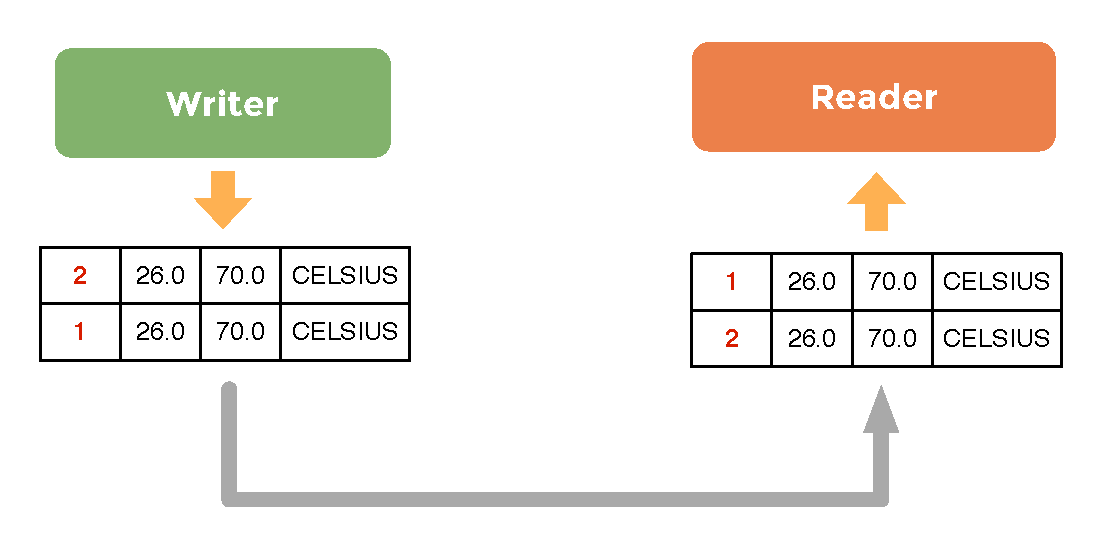
\includegraphics[scale=0.5]{figs/keyless-topic.eps}
	\caption{Data Reader queues for a keyless Topics.}
	\label{Figure:DDS:DRCache:NoKey:Topic}
\end{figure}
%%%
If we write the same samples for the \texttt{TempSensorTopic}, 
the end-result is quite different. The two samples written in the 
code fragment below have two different id values, respectively 1 and 2, 
as a result they are referring to two different instances. 
%%%
\iftoggle{cpp}{
\lstinputlisting[
		frame=tb,
		label={Listing:DDS:CreateKeyedAndKeyLessTopics}]
		{./listing/cxx/WriteKeyedInstanceExample.cpp}
}
%%%
In this case the reader will see these two samples posted into two different queues, 
as represented in Figure~\ref{Figure:DDS:DRCache:Keyed:Topic}, one queue for each instance. 
%%%
\begin{figure}[ht]
	\centering
	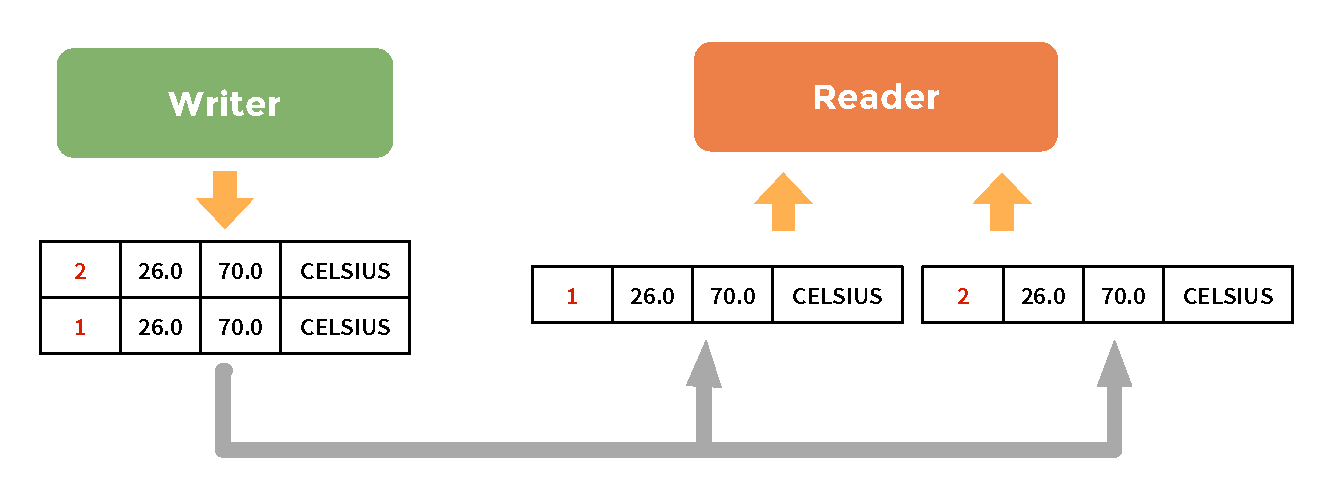
\includegraphics[scale=0.5]{figs/keyed-topic.eps}
	\caption{Data Reader queues for a keyed Topics.}
	\label{Figure:DDS:DRCache:Keyed:Topic}
\end{figure}
%%%
In summary, you should think of Topics as classes in an object oriented 
language and understand that each unique key-value identifies an instance. 
The life-cycle of topic instances is managed by DDS and to each topic instance 
are associated memory resources, you can think of it as a queue on the reader side.  
Keys identify specific data streams within a Topic. Thus, in our running example, 
each id value will identify a specific temperature sensor. 
Differently from many other \ac{Pub/Sub} technologies, \ac{DDS} allows you to 
use keys to automatic demultiplex different streams of data. 
Furthermore, since each temperature sensor will be representing an instance of 
the \texttt{TempSensorTopic} you'll be able to track the lifecycle of the sensor 
by tracking the lifecycle of its associated instance. 
You can detect when a new sensor is added into the system, just because 
it will introduce a new instance, you can detect when a sensor has failed, 
thanks to the fact that DDS can inform you when there are no more writers for a 
specific instance. You can even detect when a sensor has crashed and then recovered 
thanks to some information about the state transition that are provided by \ac{DDS}. 

Finally, before setting to rest \ac{DDS} instances, I want to underline 
that \ac{DDS} subscriptions concerns Topics. As a result when subscribing to a topic, 
you'll receive all the instances produced for that topic.  In some cases this is 
not desirable and some scoping actions are necessary. Let's see then what DDS has to offer.

\section{Scoping Information}\label{Section:Scoping:Information}
\subsection{Domain}
DDS provides two mechanism for scoping information, domains and partitions.
A domain establishes a virtual network linking all the \ac{DDS} applications 
that have joined it. 
No communication can ever happen across domains unless explicitly mediated 
by the user application. 
\subsection{Partition}
Domains can be further organized into partitions, where each partition represent 
a logical grouping of topics. DDS Partitions are described by names such 
as "SensorDataPartition", "CommandPartition", "LogDataPartition", etc., 
and have to be explicitly joined in order to publish data in it or subscribe 
to the topics it contains. The mechanism provided by \ac{DDS} for joining a 
partition is very flexible as a publisher or a subscriber can join by providing 
its full name, such as "SensorDataPartition" or it can join all the partitions 
that match a regular expression, such as "Sens*", or "*Data*". 
Supported regular expressions are the same as those accepted by the POSIX 
\texttt{fnmatch} \cite{POSIX:fmatch} function. 

To recap, partitions provide a way of scoping information. 
You can use this scoping mechanism to organize topics into different coherent sets. 
You can equally use partitions to segregate topic instances.  
Instance segregation can be necessary for optimizing performance or minimizing 
footprint for those applications that are characterized by a very large number 
of instances, such as large telemetry systems, or financial trading applications.
If we take as an example our temperature monitoring and control system, 
then we can devise with a very natural partitioning of data that mimics the 
physical placement of the various temperature sensors.  To do this, we can use 
a partition naming scheme made of the building number, the floor level and the 
room number in which the sensor is installed:
\begin{center}
  \texttt{"building-<number>:floor-<level>:room-<number>"}
\end{center}
Using this naming scheme, as shown in Figure~\ref{Figure:DDS:Partitions}, 
all the topics produced 
in room 51 on the 15th floor on building 1 would belong to the partition 
\texttt{"building-1:floor-15:room-51"}. Likewise, the partition expression 
\texttt{"building-1:floor-1:room-*"} matches all the partitions for the rooms at 
the first floor in building.
%%%
\begin{figure}[t]
	\centering
	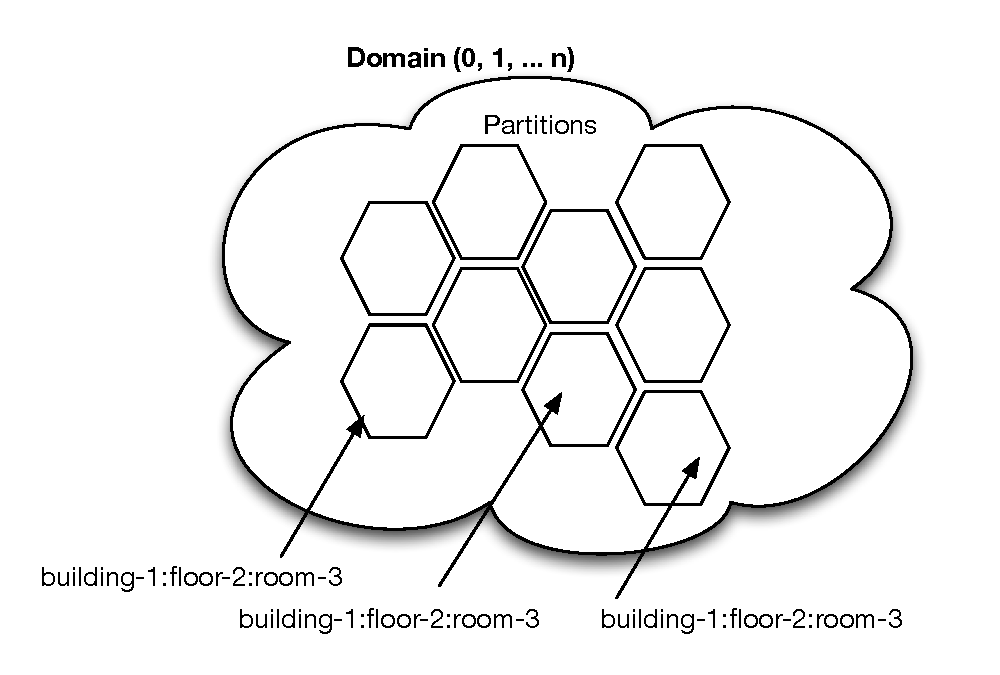
\includegraphics[scale=0.7]{figs/domain-partitions.eps}
	\caption{Domain and partitions in DDS.}
	\label{Figure:DDS:Partitions}
\end{figure}
%%%

In a nutshell,  you can use partitions to scope information, you can also 
use naming conversions such as those used for our temperature control 
applications to emulate hierarchical organization of data starting from 
flat partitions. Using the same technique you can slice and access data 
across different dimensions or views, depending on the need of your application.
%%%
%%%
%%%
\section{Content Filtering}~\label{Section:Content:Filtering}
Domains and Partitions are useful mechanisms for structurally organizing data, 
but what if you need to control the data received based on its content? 
Content Filtering allows you to create topics that constrain the 
values their instances might take. When subscribing to a content-filtered 
topic an application will only receive, among all published values, 
only those that match the topic filter.  The filter expression can 
operate on the full topic content, as opposed to being able to operate 
only on headers as it happens in many other pub/sub technologies, 
such as JMS. The filter expression is structurally similar to a SQL WHERE clause.
The operators supported by are listed in Table~\ref{Table:DDS:Filter:Expression}.
%%%
%%%

\begin{table}
\begin{center}
{\footnotesize\ttfamily
\begin{tabular}{|c|l|} \hline
\textbf{Constructed Type} 	&  	\textbf{Example}  			\\ \hline
              =           	&  	equal  						\\ \hline
              <>          	&  	not equal					\\ \hline
              >           	&  	greater than  				\\ \hline
              <				& 	less than					\\ \hline
              >=				& 	greater than or equal 		\\ \hline
              <=				&	less than or equal			\\ \hline
              BETWEEN		&   between and inclusive range	\\ \hline
              LIKE			&	matches a string pattern		\\ \hline               
\end{tabular}}
\end{center}
\label{Table:DDS:Filter:Expression}
\caption{Legal operators for  DDS Filters and Query Conditions}
\end{table}
%%%
%%%
%%%
Content-Filtered topics are very useful from several different perspectives. 
First of all they limit the amount of memory used by \ac{DDS} to the 
instances and samples that match the filter.  Furthermore, filtering can be 
used to simplify your application by delegating to DDS the logic that checks 
certain data properties. For instance, if we consider our temperature control 
application we might be interested in being notified only then the temperature 
or the humidity are outside a given range. 
Thus assuming we wanted to maintain the temperature between $20.5\,^{\circ}\mathrm{C}$ and 
$21.5\,^{\circ}\mathrm{C}$ and the humidity between $30\%$ and $50\%$, 
we could create a Content-Filtered topic that would alert the application when the 
sensor is producing value outside our desired set point.  This can be done by using the 
filter expression below:
%%%

\begin{lstlisting}[frame=tb]
       ((temp NOT BETWEEN (20.5 AND 21.5)) 
          OR 
       (hum NOT BETWEEN (30 AND 50)))
\end{lstlisting}
%%%
Listing~\ref{Listing:DDS:ContentFiltered:Topic} shows the code that creates a 
content-filtered topic for the TempSensor topic  with the expression above. 
Notice that the content-filtered topic is created starting from a regular topic. 
Furthermore it is worth noticing that the filter expression  is relying on positional 
arguments $\%0$, $\%2$, etc., whose actual values are passed via a vector of strings. 

%%%
\iftoggle{cpp}{
	\lstinputlisting[
		frame=b,
		label={Listing:DDS:ContentFiltered:Topic},
		caption={Content Filtered Topic.}]
		{./listing/cxx/content-filtered-topic.cpp}
}
%%%


\section{Summary}
In this chapter I have covered the most important aspects of data management in DDS. 
By now you've learned all you needed to know about topics-types and topic instances 
and you've been exposed to the the various mechanism provided by DDS for scoping 
information. In summary, you can organize structurally your information by means 
of domains and partitions. Then you can create special views using content-filtered 
topics and query conditions.
At this point my usual suggestion is that you try to compile and run the examples 
and try to experiment a bit by yourself.


\chapter{Reading and Writing Data}\label{Chapter:Read:Write:Data} \index{Data Reader} \index{DataWriter}
In the previous chapter I covered the definition and semantics of DDS topics, 
topic-instances and samples. I also went through domains and partitions 
and the role they play in organizing application data flows. 
In this chapter I'll examine the mechanisms provided by DDS for 
reading and writing data. 

\section{Writing Data}\label{Section:Writing:Data} \index{Data Reader}
As you've seen in the first two chapters, writing data 
with \ac{DDS} is as simple as calling the write method on the 
\texttt{DataWriter}. Yet, to make you into a fully proficient \ac{DDS} 
programmer there are a few more things you should know. 
Most notably, the relationship between writers and topic-instances life-cycle.
To explain the difference between topics and topic instances I drew the 
analogy between \ac{DDS} topics/topic-instances and classes/objects in an 
Object Oriented Programming language, such as Java or C++. Like objects,  
topic-instances have (1) an identity provided by their unique key value, 
and (2) a life-cycle. The topic-instance life-cycle can be implicitly 
managed through the semantics implied by the \texttt{DataWriter}, or it 
can be explicitly controlled via the \texttt{DataWriter} API.
The topic-instances life-cycle transition can have implications on 
local and remote resource usage, thus it is important that you understand 
this aspect.

\subsection{Topic-Instances Life-cycle} \index{Topic Instance} \index{Instance life-cycle management}
Before getting into the details of how the life-cycle is managed, 
let's see which are the possible states. A topic instance is 
\texttt{ALIVE} if there is at least one \texttt{DataWriter} that has
explicitly or implicitly (through a write) registered it.
An instance is in the \texttt{NOT\_ALIVE\_NO\_WRITERS} 
state when there are no more \texttt{DataWriters} writing it. 
Finally, the instance is \texttt{NOT\_ALIVE\_DISPOSED} 
if it was disposed either implicitly, due to some default \ac{QoS} 
settings, or explicitly, by means of a specific \texttt{DataWriter}
API call. The \texttt{NOT\_ALIVE\_DISPOSED} state indicates that the 
instance is no more relevant for the system and that it won't be 
written anymore (or any-time soon) by any writer.  
As a result the resources allocated throughout the system for storing 
the instance can be freed.  Another way of thinking about this, 
is that an instance defines a live data element in the \ac{DDS} global 
data space as far as there are writers for it. This data element ceases 
to be alive when there are no more writers for it. Finally, once 
disposed this data entity can be reclaimed from the \ac{DDS} global 
data space, thus freeing resources.  

\subsection{Automatic Life-cycle Management}
Let's try to understand the instances life-cycle management with an example. 
If we look at the code in Listing~\ref{Listing:DDS:Auto:Instance:Management}, 
and assume this is the only 
application writing data, the result of the three write operations is 
to create three new topic instances in the system for the key 
values associated with the $id = 1,  2,  3$ (we defined the \texttt{TempSensorType}
in the first installment as having  a single attribute key named id).  
These instances will be in the \texttt{ALIVE} state as long as this application 
will be running, and will be automatically registered, we could say 
associated, with the writer. The default behavior for DDS is then to 
dispose the topic instances once the \texttt{DataWriter} object is 
destroyed, thus leading the instances to the \texttt{NOT\_ALIVE\_DISPOSED} 
state. The default settings can be overridden to simply induce instances' 
unregistration, causing in this case a transition from \texttt{ALIVE} to 
\texttt{NOT\_ALIVE\_NO\_WRITERS}.

\lstinputlisting[
		frame=b,
		label={Listing:DDS:Auto:Instance:Management},
		caption={Automatic management of Instance life-cycle.}]
		{./listing/cxx/auto-instance-lifecycle.cpp}


\subsection{Explicit Life-cycle Management}
Topic-instances life-cycle can also be managed explicitly via the API
defined on the \texttt{DataWriter}. In this case the application programmer 
has the control on when instances are registered, unregistered and disposed. 
Topic-instances registration is a good practice to follow whenever an 
applications writes an instance very often and requires the lowest latency 
write. In essence the act of explicitly registering an instance allows the 
middleware to reserve resources as well as optimize the instance lookup. 
Topic-instance unregistration provides a mean for telling \ac{DDS} that an 
application is done with writing a specific topic-instance, thus all the  
resources locally associated with can be safely released. Finally,  
disposing topic-instances gives a way of communicating DDS that the instance 
is no more relevant for the distributed system, thus whenever possible resources 
allocated with the specific instances should be released both locally and remotely.
Listing 2 shows and example of how the DataWriter API can be used to register, 
unregister and dispose topic-instances.  In order to show you the full life-cycle 
management I’ve changed the default DataWriter behavior to avoid that instances 
are automatically disposed when unregistered. In addition, to maintain the code 
compact I take advantage of the new C++11 \texttt{auto} feature which leaves it to the  
the compiler to infer the left hand side types from the right hand side 
return-type. Listing 2 shows an application that writes four samples belonging 
to four different topic-instances, respectively those with $id=0,1,2,3$.  
The instances with $id=1,2,3$ are explicitly registered by calling the 
\texttt{DataWriter::register\_instance} method, while the instance with $id=0$ 
is automatically registered as result of the write on the \texttt{DataWriter}. 
To show the different possible state transitions, the topic-instance 
with $id=1$ is explicitly unregistered thus causing it to transition to 
the \texttt{NOT\_ALIVE\_NO\_WRITER} state; the topic-instance with $id=2$ 
is explicitly disposed thus causing it to transition to the 
\texttt{NOT\_ALIVE\_DISPOSED} state.  Finally, the topic-instance with 
$id=0,3$ will be automatically unregistered, as a result of the destruction 
of the objects $dw$ and $dwi3$ respectively, thus transitioning to the state 
\texttt{NOT\_ALIVE\_NO\_WRITER}. Once again, as mentioned above, in this 
example the writer has been configured to ensure that topic-instances are 
not automatically disposed upon unregistration.

\subsection{Keyless Topics} \index{Keyless Topics}
Most of the discussion above has focused on keyed topics, but what about 
keyless topics? 
As explained in chapter~\ref{Chapter:Topics:Domain:Partitions}, 
keyless topics are like singletons, in the sense that there is only one instance. 
As a result for keyless topics the the state transitions are tied to the 
lifecycle of the data-writer.
%%%
\lstinputlisting[
		frame=b,
		label={Listing:DDS:Manual:Instance:Management},
		caption={Explicit management of topic-instances life-cycle.}]
		{./listing/cxx/manunal-instance-lifecycle.cpp}
%%%
\subsection{Blocking or Non-Blocking Write?}
One question that you might have at this point is whether the write 
is blocking or not. The short answer is that the write is non-blocking, 
however, as we will see later on, there are cases 
in which, depending on \ac{QoS} settings, the write might block. 
In these cases, the blocking behaviour is necessary to avoid 
avoid data-loss. 


\section{Accessing Data}
\ac{DDS} provides a mechanism to select the samples based 
on their content and state and another to control whether 
samples have to be read or taken (removed from the cache). 

\subsection{Read vs. Take}\index{read and take operations}
The \ac{DDS} provides data access through the \texttt{DataReader} class which 
exposes two semantics for data access: read and the take.
The read semantics, implemented by the \texttt{DataReader::read} methods, 
gives access to the data received by the \texttt{DataReader} without removing 
it from its cache. This means that the data will be again readable 
via an appropriate read call. Likewise, the  take 
semantics, implemented by the \texttt{DataReader::take} method, 
allows to access the data received by the \texttt{DataReader} by removing 
it from its local cache. This means that once the data is taken, it is 
no more available for subsequent read or take operations.
The semantics provided by the  read and take operations allow you to 
use \ac{DDS} as either a distributed cache or like a queuing system, or both.
This is a powerful combination that is rarely found in the same middleware platform. 
This is one of the reasons why \ac{DDS} is used in a variety of systems 
sometimes as a high-performance distributed cache, other like a high-performance 
messaging technology, and yet other times as a combination of the two. 
In addition, the read semantics is useful when using topics to model 
distributed state, while the take semantics when modeling distributed events.

\subsection{Data and Meta-Data} \index{Data} \index{Meta-Data}
In the first part of this chapter I showed how the \texttt{DataWriter} 
can be used to control the life-cycle of  topic-instances.  
The topic-instance life-cycle along with other information describing properties 
of received data samples are made available to \texttt{DataReader} and can be used 
to select the data access via either a read or take. 
Specifically, each data sample received by a \texttt{DataWriter} has
associated a \texttt{SampleInfo} describing the property of 
that sample. These properties includes information on:
\begin{itemize}
	\item \textbf{Sample State}. The sample state can be \texttt{READ} 
	or \texttt{NOT\_READ} depending on whether the sample has already 
	been read or not. 

	\item \textbf{Instance State.} As explained above, this indicates the 
	status of the instance as being either \texttt{ALIVE}, 
	\texttt{NOT\_ALIVE\_NO\_WRITERS}, or \texttt{NOT\_ALI\-VE\_DISPOSED}.
	
	\item \textbf{View State.} The view state can be \texttt{NEW} or 
	\texttt{NOT\_NEW} depending on whether this is the first sample 
	ever received for the given topic-instance or not.
\end{itemize}
The \texttt{SampleInfo} also contains a set of counters that allow to 
reconstruct the number of times that a topic-instance has performed 
certain status transition, such as becoming alive after being disposed. 
Finally, the \texttt{SampleInfo} contains a \texttt{timestamp} for the 
data and a flag that tells wether the associated data sample is valid or not.  
This latter flag is important since DDS might generate valid samples info 
with invalid data to inform about state transitions such as an instance 
being disposed.

\subsection{Selecting Samples} \index{Samples Selection} \index{Selector API}
Regardless of whether data are read or taken from \ac{DDS}, the same 
mechanism is used to express the sample selection. Thus, for brevity, 
I am going to provide some examples using the \texttt{read} operation
yet if you want to use the \texttt{take} operation you simply have to 
replace each occurrence of a \texttt{take} with a \texttt{read}. 

\ac{DDS} allows you to select data based on state and content. State-based 
selection predicates on the values of the view state, instance state and sample state.
Content-based selection predicates on the content of the sample. 

\subsubsection{State-based Selection} \index{State based selection}
For instance, 
if I am interested in getting all the data received, no matter what the view, 
instance and sample state would issue read (or a take) as follows:

\begin{lstlisting}[frame=tb]
  LoanedSamples<TempSensorType> samples = 
  	dr.select()
  		.state(DataState.any())
  		.read();
\end{lstlisting}

If on the other hand I am interested in only reading (or taking) 
all samples that have not been read yet, I would issue a read (or take) 
as follows:

\begin{lstlisting}[frame=tb]
  LoanedSamples<TempSensorType> samples = 
  	dr.select()
  		.state(SampleState.any() << SampleSate.not_read())
  		.read();
\end{lstlisting}

If I want to read new valid data, meaning no samples with only a valid \texttt{SampleInfo}, I would  issue a read (or take) as follows: 

\begin{lstlisting}[frame=tb]
  LoanedSamples<TempSensorType> samples = 
  	dr.select()
  		.state(DataState.new_data())
  		.read();
\end{lstlisting}

Finally, if I wanted to only read data associated to instances that are making 
their appearance in the system for the first time, I would issue a read (or take) as follows:

\begin{lstlisting}[frame=tb]
  LoanedSamples<TempSensorType> samples = 
  	dr.select()
  		.state(DataState(SampleState.not_read(), 
  		                 ViewState.new(), 
  		                 InstanceState.alive())
  		.read();
\end{lstlisting}

Notice that with this kind of read I would only and always get the 
first sample written for each instance, that's it. Although it might 
seem a strange use case, this is quite useful for all those applications 
that need to do something special whenever a new instance makes its appearance 
in the system for the first time. An example could be a new airplane entering a  
new region of control, in this case the system might have to do quite a few things 
that are unique to this specific state transition. 

It is also worth mentioning that if the status is omitted, and a read (or a take) is issued as follows:

\begin{lstlisting}[frame=tb]
  auto samples = dr.read();
\end{lstlisting}



This is equivalent to selecting samples with the 
\texttt{NOT\_READ\_SAMPLE\_STATE}, \texttt{ALIVE\_INSTANCE\_STATE} and \texttt{ANY\_VIEW\_STATE}.

As a final remark, it is worth pointing out that statuses allow you to select
data based on its meta-information.  

\subsubsection{Content-based Selection} \index{Content based selection}
Content-based selection is supported by \ac{DDS} through queries. 
Although the idea of a query could seem overlapping with that of content-filtering
(see section~\label{Section:Content:Filtering}) the underlying idea is different.
Filtering is about controlling the data received by the data reader -- the data that does
not matches the filter is not inserted in the data reader cache. On the other hand,
queries are about selecting the data that is in the data reader cache.

The syntax supported by query expression is identical to that used to define 
filter expression and for convenience is reported on Table~\ref{Table:DDS:Query:Expression}. 
%%%
\begin{table}
\begin{center}
{\footnotesize\ttfamily
\begin{tabular}{|c|l|} \hline
\textbf{Constructed Type} 	&  	\textbf{Example}  			\\ \hline
              =           	&  	equal  						\\ \hline
              <>          	&  	not equal					\\ \hline
              >           	&  	greater than  				\\ \hline
              <				& 	less than					\\ \hline
              >=				& 	greater than or equal 		\\ \hline
              <=				&	less than or equal			\\ \hline
              BETWEEN		&   between and inclusive range	\\ \hline
              LIKE			&	matches a string pattern		\\ \hline               
\end{tabular}}
\end{center}
\label{Table:DDS:Query:Expression}
\caption{Legal operators for content query.}
\end{table}
%%%

The execution of the query is completely 
under the user control and executed in the context of a \texttt{read} or 
\texttt{take} operation as shown in Listing~\ref{Listing:DDS:Query}.  


%%%
\iftoggle{cpp}{
	\lstinputlisting[
		frame=b,
		label={Listing:DDS:Query},
		caption={Content Query.}]
		{./listing/cxx/query.cpp}
}

%%%
%%%
\subsubsection{Instance-based Selection} \index{Instance based selection}
In some instances you may want to only look at the data coming from a specific
topic instance. As instances are identified by value of the key attributes you
may be tempted to use content filtering discriminate among them. Although this 
would work perfectly fine, it is not the most efficient way of selecting an
instance. \ac{DDS} provide another mechanism, that allows you to pinpoint the instance
you are interested in a more efficient manner than content filtering. 
In essence, each instance has associated an instance handle, this can be used 
to access the data from a given instance in a very efficient manner.

Listing~\ref{Listing:DDS:Instance:Selection} shows how this can be done.

%%%
\iftoggle{cpp}{
	\lstinputlisting[
		frame=b,
		label={Listing:DDS:Instance:Selection},
		caption={Instance-based selection.}]
		{./listing/cxx/instance-selection.cpp}
}

\subsection{Iterators or Containers?} \index{Iterators and Containers}
The examples we have seen so far where loaning the data from DDS, in other terms
you did not have to provide the storage for the samples. The advantage of 
this style of read is allows zero copy reads. However, if you want to store the 
data in a container of your choice you can use the iterator based read/take operations.
as iterator-based reads and takes. 

The iterator-based read/take API supports both forward iterators as well as 
back-inserting iterators. These API allows you to read (or take) data into 
whatever structure you'd like, as far as you can get a forward or a back-inserting 
iterator for it. If we focus on the forward-iterator based API, the back-inserting 
is pretty similar, then you might be able to read data as follows:


\begin{lstlisting}[frame=tb]
   Sample<TempSensorType>* samples = ...; // Get hold of some memory
   uint32_t n = dr.read(samples, max_samples);
   
   std::vector<Sample<TempSensorType> vsamples(max_samples);
   n = dr.read(vsamples.begin(), max_samples);
\end{lstlisting}

\subsection{Blocking or Non-Blocking Read/Take?} 
The DDS read and take are always non-blocking. If no data is available to read 
then the call will return immediately. Likewise if there is less data than requested 
the call will gather what available and return right away. The non-blocking nature of 
read/take operations ensures that these can be safely used by applications that poll 
for data.

\section{Waiting and being Notified}
One way of coordinating with DDS is to have the application poll for data 
by performing either a read or a take every so often. Polling might be the 
best approach for some classes of applications, the most common example 
being control applications that execute a control loop or a cyclic executive.  
In general, however, applications might want to be notified of the availability 
of data or perhaps be able to wait for its availability, as opposed to poll. 
\ac{DDS} supports both synchronous and asynchronous coordination by means of 
wait-sets and listeners.

\subsection{Waitsets} \index{Waitsets}
\ac{DDS} provides a generic mechanism for waiting on conditions. 
One of the supported kind of conditions are read conditions which 
can be used to wait for the availability data on one or more 
\texttt{DataReaders}. This functionality is provided by \ac{DDS} via the 
\texttt{Waitset} class which can be seen as an object oriented version of the 
Unix \texttt{select}. 

%%%
\iftoggle{cpp}{
	\lstinputlisting[
		frame=b,
		label={Listing:DDS:Waitset},
		caption={Using WaitSet to wait for data availability.}]
		{./listing/cxx/waitset.cpp}
}


\ac{DDS} conditions can be associated with functor objects which are 
then used to execute application-specific logic when the condition 
is triggered. If we wanted to wait for temperature samples to be 
available we could create a read-condition on our \texttt{DataReader} 
by passing it a functor such as the one showed in Listing~\ref{}.  
Then as shown in Listing~\ref{Listing:DDS:Waitset}, we would create a 
\texttt{Waitset} and attach the condition to it. 
At this point, we can synchronize on 
the availability of data, and there are two ways of doing it. 
One approach is to invoke the \texttt{Waitset::wait} method which 
returns the list of active conditions. These active conditions can then be 
iterated upon and their associated functors can be executed. 
The other approach is to invoke the \texttt{Waitset::dispatch}. 
In this case the infrastructure will automatically invoke the 
functor associated with triggered conditions before unblocking. 

Notice that, in both cases, the execution of the functor happens in 
an application thread. 

\subsection{Listeners} \index{Listeners}
Another way of finding-out when there is data to be read, is 
to take advantage of the events raised by DDS and notified 
asynchronously to registered handlers.  Thus, if we wanted 
an handler to be notified of the availability of data, we would 
connect the appropriate handler with the \texttt{on\_data\_available} 
event raised by the \texttt{DataReader}. Listing~\ref{Listing:DDS:Listener} 
shows how this can be done.
%%

%%%
\iftoggle{cpp}{
	\lstinputlisting[
		frame=b,
		label={Listing:DDS:Listener},
		caption={Using a listener to receive notification of data availability.}]
		{./listing/cxx/listener.cpp}
}
%%
The \texttt{NoOpDataReaderListener} is a utility class provided by the \ac{DDS}
API that provides a trivial implementation for all the operation defined as
part of the listener. This way, you can only override those that are relevant 
for your application.

When using C++11 however it would be nice to be able to use a lambda function
to define the actions to execute to handle a specific event. Although this
feature is not currently supported by the \ac{DDS} C++ API, there are some 
libraries, such as the one available at \url{https://github.com/kydos/dds-cpp11} 
that make it possible.

%%%
\iftoggle{cpp}{
	\lstinputlisting[
		frame=b,
		label={Listing:DDS:Listener11},
		caption={Using a C++ lambda to define the action to be execute in response of a data availability notification.}]
		{./listing/cxx/listener11.cpp}
}
%%
The event handling mechanism allows you to bind anything you want 
to a \ac{DDS} event, meaning that you could bind a function, a 
class method, or a functor. The only contract you need to comply 
with is the signature that is expected by the infrastructure. 
For example,  when dealing with the \texttt{on\_data\_available} 
event you have to register a callable entity that accepts a single 
parameter of type \texttt{DataReader}. 
Finally, something worth pointing out is that the handler code 
will execute in a middleware thread. As a result, when using listeners 
you should try to minimize the time spent in the listener itself.


\section{Summary}
In this chapter I have presented the various aspects involved in writing 
and reading data with DDS. I went through the topic-instance life-cycle, 
explained how that can be managed via the \texttt{DataWriter} and showcased 
all the meta-information available to \texttt{DataReader}. I also went into 
explaining wait-sets and listeners and how these can be used to receive 
indication of when data is available. 
At this point my usual suggestion is that you try to compile and run the examples 
and try to experiment a bit by yourself.

\chapter{Quality of Service}\label{Chapter:QoS}
\section{The DDS QoS Model} \label{Section:DDS:QoS} \index{QoS Model}
\begin{figure}[t]
	\centering
	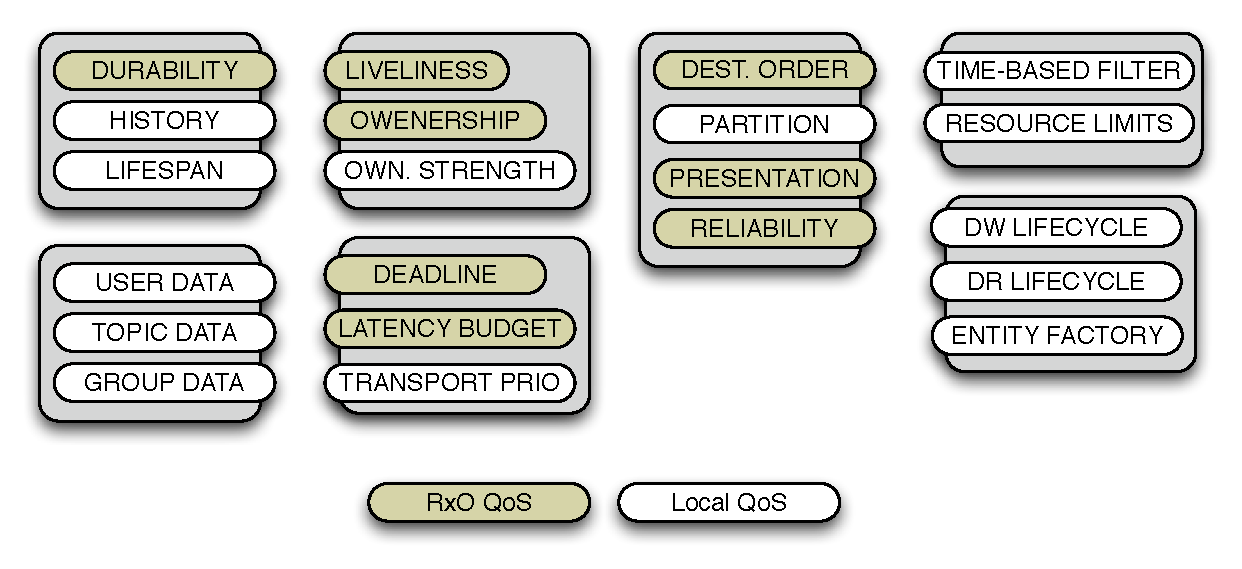
\includegraphics[scale=0.6]{figs/QoS-Map.eps}
	\caption{DDS QoS Policies.}
	\label{Figure:DDS:QoSMap}
\end{figure}
%%%
\ac{DDS} provides applications policies to control a wide set
of non-functional properties, such as data availability, data
delivery, data timeliness and resource usage -- Figure~\ref{Figure:DDS:QoSMap} shows
the full list of available QoS.  
The semantics and the behaviour of \ac{DDS} entities, such as a topic, data
reader, and data writer, can be controlled through available \ac{QoS}
policies.  The policies that control and end-to-end property are
considered as part of the subscription matching. 
%%%
\begin{figure}[t]
	\centering
	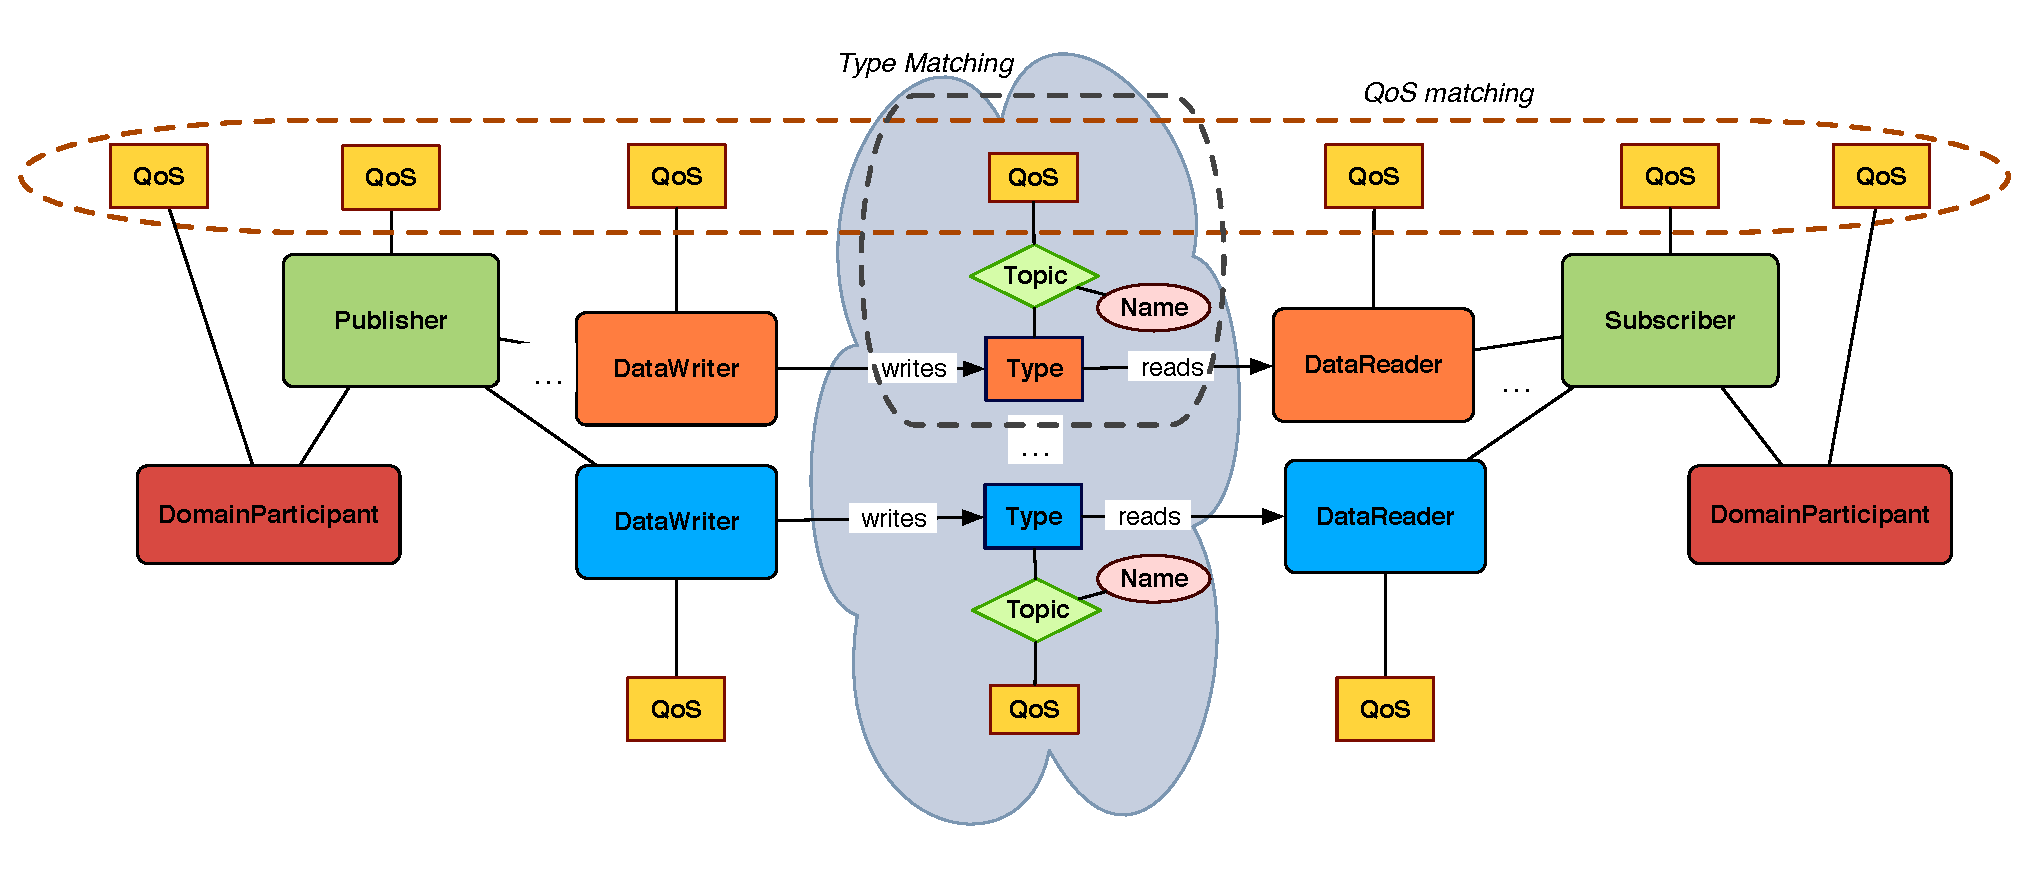
\includegraphics[scale=0.4]{figs/RxO.eps}
	\caption{DDS Request vs. Offered QoS Model.}
	\label{Figure:DDS:RxO}
\end{figure}
%%%
\ac{DDS} uses a request vs. offered QoS matching approach, as
shown in Figure~\ref{Figure:DDS:RxO} in which a
data reader matches a data writer if and only if the QoS it is
requesting for the given topic does not exceed (e.g., is no more
stringent) than the QoS with which the data is produced by the data
writer.  

\ac{DDS} subscriptions are matched against the topic type and
name, as well as against the \ac{QoS} being offered\-/requested by
data writers and readers.  This DDS matching mechanism ensures that
(1) types are preserved end-to-end due to the topic type matching and
(2) end-to-end \ac{QoS} invariants are also preserved.

The reminder of this section describes the most important \ac{QoS}
policies in \ac{DDS}.

\subsection{Data availability} \index{Data Availability QoS}
DDS provides the following QoS policies that control the availability
of data to domain participants:
\begin{itemize}

	\item The \texttt{DURABILITY} \ac{QoS} policy controls the
          lifetime of the data written to the global data space in a
          \ac{DDS} domain.  Supported durability levels include (1)
          \texttt{VOLATILE}, which specifies that once data is
          published it is not maintained by \ac{DDS} for delivery to
          late joining applications, (2) \texttt{TRANSIENT\_LOCAL},
          which specifies that publishers store data locally so that
          late joining subscribers get the last published item if a
          publisher is still alive, (3) \texttt{TRANSIENT}, which
          ensures that the \ac{GDS} maintains the information outside
          the local scope of any publishers for use by late joining
          subscribers, and (4) \texttt{PERSISTENT}, which ensures that
          the \ac{GDS} stores the information persistently so to make
          it available to late joiners even after the shutdown and
          restart of the whole system.  Durability is achieved by
          relying on a durability service whose properties are
          configured by means of the \texttt{DURABILITY\_SERVICE}
          \ac{QoS} of non-volatile topics.

	\item The \texttt{LIFESPAN} \ac{QoS} policy controls the
          interval of time during which a data sample is valid. The
          default value is infinite, with alternative values being the
          time-span for which the data can be considered valid.

	\item The \texttt{HISTORY} \ac{QoS} policy controls the number
          of data samples (i.e., subsequent writes of the same topic)
          that must be stored for readers or writers. Possible values
          are the last sample, the last $n$ samples, or all samples.
\end{itemize}
These \ac{DDS} data availability \ac{QoS} policies decouple
applications in time and space.  They also enable these applications
to cooperate in highly dynamic environments characterized by
continuous joining and leaving of publisher\-/subscribers.  Such
properties are particularly relevant in \ac{SoS} since they increase
the decoupling of the component parts.

\subsection{Data delivery} \index{Data Delivery QoS}
DDS provides the following QoS policies that control how data is
delivered and how publishers can claim exclusive rights on data
updates:
%%%
\begin{itemize}
	\item The \texttt{PRESENTATION} QoS policy gives control on
          how changes to the information model are presented to
          subscribers. This \ac{QoS} gives control on the ordering as
          well as the coherency of data updates.  The scope at which
          it is applied is defined by the access scope, which can be
          one of \texttt{INSTANCE}, \texttt{TOPIC}, or \texttt{GROUP}
          level.

	\item The \texttt{RELIABILITY} QoS policy controls the level
          of reliability associated with data diffusion. Possible
          choices are \texttt{RELIABLE} and \texttt{BEST\_EFFORT}
          distribution.

	\item The \texttt{PARTITION} \ac{QoS} policy gives control
          over the association between \ac{DDS} partitions
          (represented by a string name) and a specific instance of a
          publisher/subscriber.  This association provides \ac{DDS}
          implementations with an abstraction that allow to segregate
          traffic generated by different partitions, thereby improving
          overall system scalability and performance.
	
 	\item The \texttt{DESTINATION\_ORDER} \ac{QoS} policy controls
          the order of changes made by publishers to some instance of
          a given topic. DDS allows the ordering of different changes
          according to source or destination timestamps.

	\item The \texttt{OWNERSHIP} \ac{QoS} policy controls which
          writer ``owns'' the write-access to a topic when there are
          multiple writers and ownership is \texttt{EXCLUSIVE}. Only
          the writer with the highest \texttt{OWNERSHIP\_STRENGTH} can
          publish the data.  If the \texttt{OWNERSHIP} \ac{QoS} policy
          value is shared, multiple writers can concurrently update a
          topic. \texttt{OWNERSHIP} thus helps to manage replicated
          publishers of the same data.
	
\end{itemize}
These \ac{DDS} data delivery \ac{QoS} policies control the reliability
and availability of data, thereby allowing the delivery of the right
data to the right place at the right time.  More elaborate ways of
selecting the right data are offered by the \ac{DDS} content-awareness
profile, which allows applications to select information of interest
based upon their content.  These \ac{QoS} policies are particularly
useful in \ac{SoS} since they can be used to finely tune how---and to
whom---data is delivered, thus limiting not only the amount of
resources used, but also minimizing the level of interference by
independent data streams.

\subsection{Data timeliness} \index{Data Timeliness QoS}
DDS provides the following \ac{QoS} policies to control the timeliness
properties of distributed data:
%%%
\begin{itemize}

	\item The \texttt{DEADLINE} \ac{QoS} policy allows
          applications to define the maximum inter-arrival time for
          data. \ac{DDS} can be configured to automatically notify
          applications when deadlines are missed.

	\item The \texttt{LATENCY\_BUDGET} QoS policy provides a means
          for applications to inform \ac{DDS} of the urgency
          associated with transmitted data.  The latency budget
          specifies the time period within which \ac{DDS} must
          distribute the information. This time period starts from the
          moment the data is written by a publisher until it is
          available in the subscriber’s data-cache ready for use by
          reader(s).

	\item The \texttt{TRANSPORT\_PRIORITY} QoS policy allows
          applications to control the importance associated with a
          topic or with a topic instance, thus allowing a DDS
          implementation to prioritize more important data relative to
          less important data. These QoS policies help ensure that
          mission-critical information needed to reconstruct the
          shared operational picture is delivered in a timely manner.
\end{itemize}
These \ac{DDS} data timeliness \ac{QoS} policies provide control over
the temporal properties of data.  Such properties are particularly
relevant in \ac{SoS} since they can be used to define and control the
temporal aspects of various subsystem data exchanges, while ensuring
that bandwidth is exploited optimally.

\subsection{Resources} \index{Resource Control QoS}
\ac{DDS} defines the following \ac{QoS} policies to control the
network and computing resources that are essential to meet data
dissemination requirements:
\begin{itemize}

	\item The \texttt{TIME\_BASED\_FILTER} \ac{QoS} policy allows
          applications to specify the minimum inter-arrival time
          between data samples, thereby expressing their capability to
          consume information at a maximum rate. Samples that are
          produced at a faster pace are not delivered. This policy
          helps a \ac{DDS} implementation optimize network bandwidth,
          memory, and processing power for subscribers that are
          connected over limited bandwidth networks or which have
          limited computing capabilities.

	\item The \texttt{RESOURCE\_LIMITS} \ac{QoS} policy allows
          applications to control the maximum available storage to
          hold topic instances and related number of historical
          samples \ac{DDS}’s \ac{QoS} policies support the various
          elements and operating scenarios that constitute net-centric
          mission-critical information management. By controlling
          these QoS policies it is possible to scale \ac{DDS} from
          low-end embedded systems connected with narrow and noisy
          radio links, to high-end servers connected to high-speed
          fiber-optic networks.
\end{itemize}
These \ac{DDS} resource \ac{QoS} policies provide control over the
local and end-to-end resources, such as memory and network bandwidth.
Such properties are particularly relevant in \ac{SoS} since they are
characterized by largely heterogeneous subsystems, devices, and
network connections that often require down-sampling, as well as
overall controlled limit on the amount of resources used.

\subsection{Configuration} \index{Configuration QoS}
The \ac{QoS} policies described above, provide control over the most
important aspects of data delivery, availability, timeliness, and
resource usage.  \ac{DDS} also supports the definition and
distribution of user specified bootstrapping information via the
following QoS policies:

\begin{itemize}
%%%
	\item The \texttt{USER\_DATA} \ac{QoS} policy allows
          applications to associate a sequence of octets to domain
          participant, data readers and data writers. This data is
          then distributed by means of a built-in topic. This QoS
          policy is commonly used to distribute security credentials.

	\item The \texttt{TOPIC\_DATA} \ac{QoS} policy allows
          applications to associate a sequence of octet with a
          topic. This bootstrapping information is distributed by
          means of a built-in topic. A common use of this \ac{QoS}
          policy is to extend topics with additional information, or
          meta-information, such as IDL type-codes or XML schemas.

	\item The \texttt{GROUP\_DATA} \ac{QoS} policy allows
          applications to associate a sequence of octets with
          publishers and subscribers--this bootstrapping information
          is distributed by means built-in topics.  A typical use of
          this information is to allow additional application control
          over subscriptions matching.
\end{itemize}
These \ac{DDS} configuration \ac{QoS} policies provide useful a
mechanism for bootstrapping and configuring applications that run in
\ac{SoS}.  This mechanism is particularly relevant in \ac{SoS} since
it provides a fully distributed means of providing configuration
information.


\subsection{Setting QoS}
All the code examples you have have seen so far did rely on default \ac{QoS} 
settings, as such we did not have to be concerned with defining the desired 
\ac{QoS}. Listing~\ref{Listing:DDS:QoS} shows how you can create and set 
\ac{QoS} on \ac{DDS} entities. 


%%%
%%%
\iftoggle{cpp}{
	\lstinputlisting[
		frame=b,
		label={Listing:DDS:QoS},
		caption={Setting QoS on DDS entities.}]
		{./listing/cxx/qos-example.cpp}
}
%%%

Along with an API to explicitly create \ac{QoS}, \ac{DDS} also provides
the concept of a \texttt{QoSProvider} to make it possible to externalize the 
definition of the \ac{QoS} and make it a deployment time concern.
The listing below show how the \texttt{QoSProvider} can be used to fetch
\ac{QoS} definition from a file. 

%%%
\iftoggle{cpp}{
	\lstinputlisting[
		frame=b,
		label={Listing:DDS:QoS},
		caption={Setting QoS on DDS entities using the QoSProvider.}]
		{./listing/cxx/qos-provider.cpp}
}
%%%

\section{Summary}
In this chapter I've explained the role of \ac{QoS} in \ac{DDS} and shown how 
the various policies can be used to control the most important aspects of 
communication, data availability and resource usage. 
The code example have also illustrated that setting \ac{QoS} is pretty straightforward
and the use of the \texttt{QoSProvider} can be of great help in making the selection
of \ac{QoS} a deployment concern.

\appendix
\chapter{Online Resources}~\label{Appendix:A}
\section{Examples Source Code}
All the examples presented throughout the Tutorial are available online at 
\iftoggle{cpp}{
	\url{https://github.com/kydos/dds-tutorial-cpp}.
}

The \texttt{README.md} provides all the information necessary to install and run 
the examples.


\section{Getting a DDS Implementation}
\iftoggle{cpp}{
At the time of writing, the only open source, as well as commercial, \ac{DDS} implementation
that supports the new C++ API is \href{http://www.opensplice.org/}{OpenSplice DDS} which is 
freely available at \url{http://www.opensplice.org}.
}


\section{C++11 Considerations}
Although some of the examples in this tutorial take advantage of C++11, the new \ac{DDS} C++ API can also be used with C++03 compilers. 
That said, should you have possibility of using a C++11 compiler, then there are 
some additional aspects of the language that can be enabled. If you are interested in
learning more take a look at the following GitHub project \url{https://github.com/kydos/dds-cpp11}


\backmatter
\chapter{Acronyms}
\begin{acronym}
%%% A
 \acro{AMQP}{Advanced Message Queuing Protocol}
%%% B
%%% C
  \acro{CDR}{Common Data Representation}
%%% D
  \acro{DDS}{The Data Distribution Service}
  \acro{DDSI}{Data Distribution Service Interoperability Wire Protocol}
  \acro{DISR}{DoD Information-Technology Standards Registry}
  \acro{DoD}{Department of Defence}
  \acro{DP}{Domain Participant}
  \acro{DR}{Data Reader}
  \acro{DW}{Data Writer}
	
%%% E
%%% F
%%% G
  \acro{GDS}{Global Data Space}
%%% H
%%% I
  \acro{I2}{Industrial Internet}
  \acro{IDL}{Interface Definition Language}
  \acro{IoT}{Internet of Things}
   
%%% J
  \acro{JMS}{the Java Message Service}
%%% K
%%% L
%%% M
  \acro{MILVA}{Military Vehicle Association}
  \acro{MoD}{Mistry of Defence}
  \acro{MQTT}{Message Queuing Telemetry Transport}
%%% N
%%% O
  \acro{OMG}{Object Management Group}
  \acro{OS}{Operating System}
%%% P
  \acro{Pub/Sub}{Publish/Subscribe}
%%% Q
  \acro{QoS}{Quality of Service}
%%% R
%%% S
  \acro{SoS}{Systems-of-Systems}
%%% T
%%% U
  \acro{ULS}{Ultra Large Scale Systems}
  \acro{UML}{Unified Modeling Langauge}
%%% V
%%% W
%%% X
  \acro{XML}{eXtensible Markup Langauge}
%%% Y
%%% Z
\end{acronym}

%%%
%%% Index
%%%
\printindex
%%%
%%% Bibliography
%%%
\bibliography{biblio}{ }
\bibliographystyle{plain}

\end{document}
